\section{General compiler}
% möjlig ref till drakboken
New languages are often developed to allow for a higher level of abstraction and a higher level of reasoning about algorithms. To be able to run these new languages compilers are built to convert the high level code down to machine code, to run directly on hardware, or to a lower level language to make use of that language's compiler. 

\begin{figure}[!ht]
  \centering
  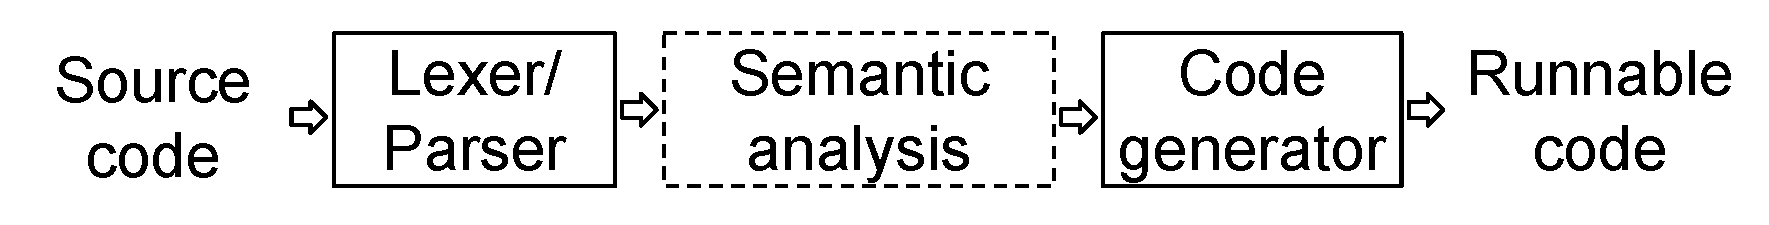
\includegraphics[width=0.6\pdfpagewidth]{figure/generalpipeline}
  \caption{A general compiler pipeline}
  \label{fig:generalpipeline}
\end{figure}

The structure of a compiler can be likened to a pipe where text flows through. 
The text flowing through the pipe is transformed between different representations and is in
the end output as runnable code to either run on the computer itself or on a virtual machine
that emulates a computer. 

\todo{Read and improve!}
To ensure that the compiled program is correct and does not do anything nonsencical \todo{change nonsensical? what do we mean? nonsensical might need a context for the reader if we keep it}, analysis is done on the code. This could be a call graph \todo{is call graph a too difficult example? will the reader understand?} to remove dead code or making sure that a variable is defined before use. Hopper, and Haskell somewhat famously, performs type checking, which is showing correctness by proving types.

In figure ~\ref{fig:generalpipeline} you can see the flow handling the source code.
It should be noted that the semantic analysis is optional for a language, it can
fully rely on the grammar to expose errors. This will lead to a more expressive, 
or less restricted, language but increases the risk of runtime crashes due to type errors.

We start by describing the first step of a compiler, the lexer and parser.
